\documentclass[11pt, letterpaper]{article}

% ── Packages ──
\usepackage[margin=0.8in]{geometry}
\usepackage{amsmath, amssymb, amsthm}
\usepackage{graphicx}
\usepackage{booktabs}
\usepackage{hyperref}
\usepackage{caption}
\usepackage{subcaption}
\usepackage{float}
\usepackage{microtype}
\usepackage{hyphenat}
\usepackage{parskip}
\usepackage{enumitem}
\usepackage[round]{natbib}

\graphicspath{{figures/}}

% ── Title ──
\title{Improving Physics-Informed Neural Networks for\\
Seismic Wave Propagation and Full Waveform Inversion}

\author{Pratham Chauhan, David Xu, Qinzhi Zhang}

\date{AMATH 445 --- Winter 2026}

\begin{document}
\maketitle

\section{Introduction}
\label{sec:intro}

Physics-informed neural networks (PINNs) \citep{raissi2019physics} embed governing PDEs directly into a neural network's loss function, enabling both forward and inverse problems to be solved in a unified, meshless optimization framework.
\citet{rashtbehesht2022} applied PINNs to the 2D acoustic wave equation for full waveform inversion (FWI), recovering subsurface wavespeed distributions from sparse surface seismograms and two early-time wavefield snapshots.
Their results are promising, but the methodology relies on hand-tuned loss weights, makes unjustified choices between activation functions across different test cases, and acknowledges but does not address the well-known spectral bias of neural networks near sharp material interfaces.
We reproduce the ellipsoidal anomaly inverse problem (Case~3) from \citet{rashtbehesht2022} and systematically evaluate four improvements:
\begin{enumerate}[nosep]
  \item Adaptive loss weighting based on gradient statistics \citep{wang2021understanding},
  \item Activation function comparison: tanh, sinusoidal/SIREN \citep{sitzmann2020implicit}, and trainable adaptive activations \citep{jagtap2020adaptive},
  \item Random Fourier feature input encoding for spectral bias mitigation \citep{tancik2020fourier},
  \item Residual-based adaptive collocation point resampling.
\end{enumerate}
We replace the original SpecFem2D ground-truth solver with a self-contained finite-difference code for full reproducibility.
The scalar acoustic wave equation in a 2D medium with negligible density variations is
\begin{equation}
  \alpha^2(x,z)\,\nabla^2 \phi = \frac{\partial^2 \phi}{\partial t^2},
  \label{eq:wave}
\end{equation}
where $\phi(x,z,t)$ is the scalar wave potential, $\alpha(x,z)$ is the spatially varying P-wave velocity, and $\nabla^2 = \partial^2/\partial x^2 + \partial^2/\partial z^2$.
For the forward problem, $\alpha$ is known and one solves for $\phi$;
for the inverse problem, $\alpha$ must be inferred from observed waveforms at sparse receiver locations.
A PINN approximates $\phi$ with a fully connected network $\hat{\phi}_\Theta(x,z,t)$.
The PDE is enforced at randomly sampled collocation points by penalizing the residual via automatic differentiation.
The total loss combines four terms:
\begin{equation}
  \mathcal{L}(\Theta) = \lambda_{\text{pde}}\mathcal{L}_{\text{pde}}
  + \lambda_{\text{snap}}\mathcal{L}_{\text{snap}}
  + \lambda_{\text{obs}}\mathcal{L}_{\text{obs}}
  + \lambda_{\text{fs}}\mathcal{L}_{\text{fs}},
  \label{eq:total-loss}
\end{equation}
where $\mathcal{L}_{\text{pde}}$ is the mean squared PDE residual, $\mathcal{L}_{\text{snap}}$ fits two early-time wavefield snapshots encoding the source, $\mathcal{L}_{\text{obs}}$ matches surface seismograms, and $\mathcal{L}_{\text{fs}}$ enforces the stress-free condition at $z=0$.
A second network $\hat{\alpha}_\Psi(x,z)$ parameterizes the unknown wavespeed; both networks are trained jointly.

\section{Methodology}
\label{sec:method}

\subsection{Ground Truth: Finite Difference Solver}
\label{sec:fd-solver}

We generate all training data using a custom 2D finite-difference solver in PyTorch with second-order central differences and explicit leapfrog time stepping ($\Delta t \leq \Delta x / (\alpha_{\max}\sqrt{2})$ for CFL stability).
Absorbing sponge layers on the left, right, and bottom boundaries prevent artificial reflections;
a stress-free condition at $z = 0$ is applied via the image method.
The source is a 20~Hz Ricker wavelet matching Case~3 of \citet{rashtbehesht2022}.
Two snapshots are taken at $t_1 = 0.100$~s and $t_2 = 0.115$~s, and 20 equally spaced surface receivers record 0.4~s of data.

\subsection{PINN Architecture}
\label{sec:architecture}

The inverse problem employs two networks trained jointly:
\begin{itemize}[nosep]
  \item \textbf{WavefieldNet} $(x,z,t) \to \phi$: 4 hidden layers of 50 neurons, tanh activation (baseline).
  \item \textbf{WavespeedNet} $(x,z) \to \alpha$: 4 hidden layers of 20 neurons, tanh activation, with output $\hat{\alpha} = \alpha_{\mathrm{bg}} + \Delta\alpha \cdot \tanh(\text{raw}) \cdot m(x,z)$, where $\alpha_{\text{bg}} = 3.0$~km/s, $\Delta\alpha = 1.0$~km/s, and $m(x,z)$ is a smooth mask restricting inversion to the domain interior.
\end{itemize}

All inputs are normalized to $[-1,1]$. The PDE residual accounts for the chain-rule scaling:
\begin{equation}
  \alpha^2 \left( s_x^2 \frac{\partial^2\phi}{\partial \hat{x}^2}
  + s_z^2 \frac{\partial^2\phi}{\partial \hat{z}^2} \right)
  = s_t^2 \frac{\partial^2\phi}{\partial \hat{t}^2},
  \label{eq:chain-rule}
\end{equation}
where $s_x = 2/L_x$, $s_z = 2/L_z$, $s_t = 2/L_t$.
Omitting these factors causes convergence to an incorrect solution, a subtlety not discussed in \citet{rashtbehesht2022}.

\subsection{Proposed Improvements}
\label{sec:improvements}

\subsubsection{Improvement 1: Adaptive Loss Weighting}
\label{sec:adaptive-weights}

We implement the gradient-balancing algorithm of \citet{wang2021understanding}, which adjusts weights dynamically:
\begin{equation}
  \hat{\lambda}_i = \frac{\max_j \|\nabla_\Theta \mathcal{L}_j\|_\infty}{\|\nabla_\Theta \mathcal{L}_i\|_\infty},
  \qquad
  \lambda_i^{(k)} = (1 - \beta)\,\lambda_i^{(k-1)} + \beta\,\hat{\lambda}_i,
  \label{eq:adaptive-weights}
\end{equation}
with $\beta = 0.1$.

\subsubsection{Improvement 2: Activation Function Study}
\label{sec:activations}

\citet{rashtbehesht2022} use sin activations for some cases and tanh for others without justification.
We compare: (a)~\textbf{tanh} (baseline), (b)~\textbf{sin} (SIREN, $\omega_0 = 30$) following \citet{sitzmann2020implicit}, and (c)~\textbf{adaptive tanh} of the form $\tanh(n \cdot a \cdot x)$ with trainable $a$ initialized to 1.0 and $n = 5$, following \citet{jagtap2020adaptive}.

\subsubsection{Improvement 3: Fourier Feature Encoding}
\label{sec:fourier}

Following \citet{tancik2020fourier}, we apply a random Fourier feature mapping:
\begin{equation}
  \gamma(\mathbf{v}) = \bigl[\cos(2\pi \mathbf{B}\mathbf{v}),\;
\sin(2\pi \mathbf{B}\mathbf{v})\bigr],
  \qquad \mathbf{B} \sim \mathcal{N}(0, \sigma^2),
  \label{eq:rff}
\end{equation}
with $\sigma = 4.0$ and 64 features (mapping 3D input to 128 dimensions).

\subsubsection{Improvement 4: Residual-Based Adaptive Collocation}
\label{sec:adaptive-colloc}

Every 500 epochs, we evaluate the PDE residual on 200{,}000 candidate points and resample $N_{\text{pde}} = 10{,}000$ collocation points: 50\% with probability proportional to the local residual magnitude, 50\% uniform.

\section{Experimental Setup}
\label{sec:setup}

All experiments use the same inverse problem: an ellipsoidal anomaly ($\alpha = 2.5$~km/s) in a 3.0~km/s background on a $1.4 \times 0.5$~km domain, matching Case~3 of \citet{rashtbehesht2022}.
Each experiment modifies exactly one component relative to the baseline.
All runs use identical random seeds and are trained for 30{,}000 epochs.
We report wavespeed RMSE and relative $L^2$ displacement error at $t = 0.250$~s.
All training was performed on a single NVIDIA RTX 4070 GPU. Hyperparameters are listed in Table~\ref{tab:hyperparams}.
\begin{table}[h]
\centering
\caption{Training hyperparameters (shared across all experiments unless noted).}
\label{tab:hyperparams}
\begin{tabular}{@{}ll@{}}
\toprule
Parameter & Value \\
\midrule
Learning rate & $10^{-3}$ (cosine decay $\to 10^{-5}$) \\
Optimizer & Adam \\
Epochs & 30{,}000 \\
$N_{\text{pde}}$ / $N_{\text{snap}}$ / $N_{\text{obs}}$ / $N_{\text{fs}}$ & 10{,}000 / 3{,}600 / 13{,}580 / 5{,}000 \\
Gradient clipping & $\|\cdot\|_2 \leq 1.0$ \\
Baseline $(\lambda_{\text{pde}}, \lambda_{\text{snap}}, \lambda_{\text{fs}}, \lambda_{\text{obs}})$ & $(0.1, 1.0, 0.1, 1.0)$ \\
\bottomrule
\end{tabular}
\smallskip

\noindent\small The baseline loss weights were adopted from \citet{rashtbehesht2022}.
\end{table}

\section{Results}
\label{sec:results}

\subsection{Baseline Reproduction}
\label{sec:baseline-results}

The baseline PINN successfully identifies the anomaly location, achieving a wavespeed RMSE of 0.190~km/s (Figure~\ref{fig:baseline}).
The velocity reduction is underestimated ($\sim$2.82~km/s predicted vs.\ 2.5~km/s true) and the boundary is smoothed.
The wavefield captures the general propagation structure but with large amplitude errors (relative error 0.875), particularly behind the wavefront where scattering produces complex interference.
\begin{figure}[H]
  \centering
  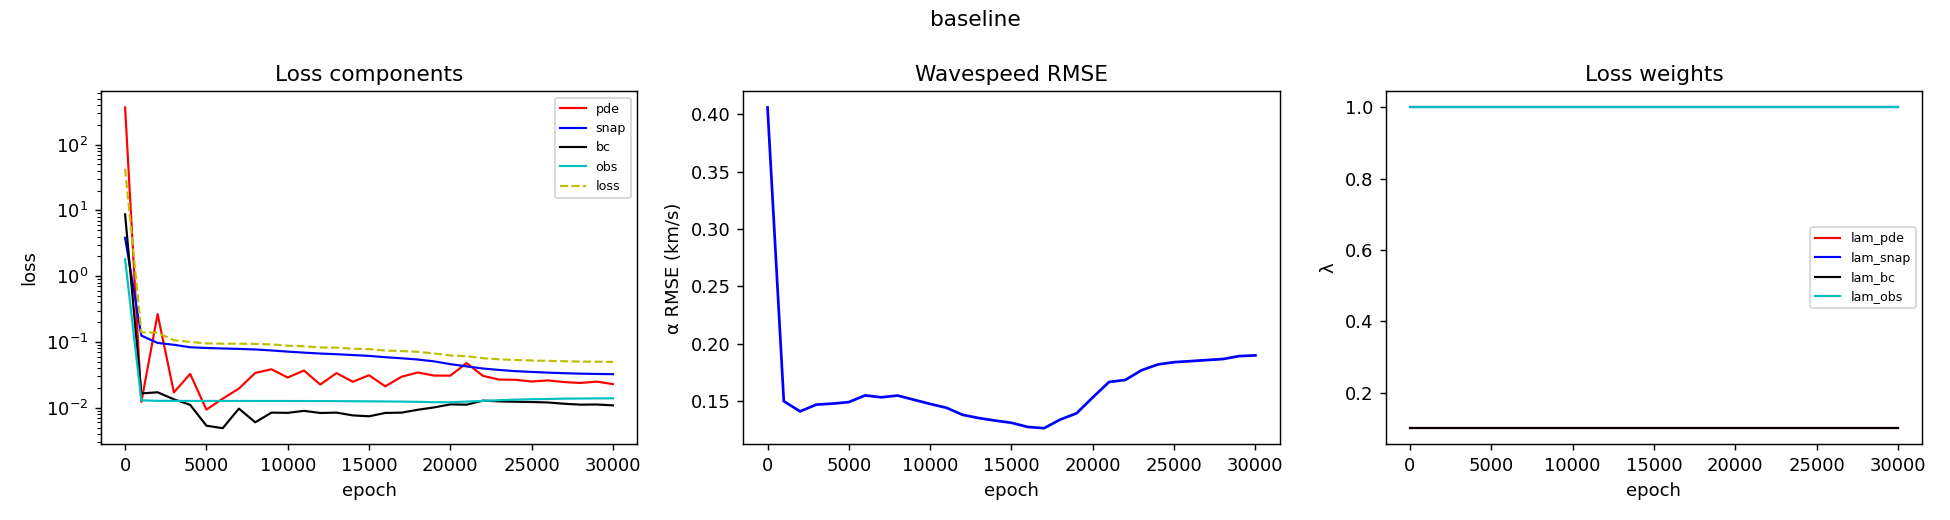
\includegraphics[width=0.8\textwidth]{baseline_final.png}
  \caption{Baseline results. Top: true wavespeed (left), predicted (center), absolute error (right; RMSE = 0.190~km/s).
Bottom: FD wavefield at $t = 0.250$~s (left), PINN prediction (center), error (right; rel.\ err = 0.875).}
  \label{fig:baseline}
\end{figure}

\subsection{Effect of Individual Improvements}
\label{sec:improvement-results}

Table~\ref{tab:results} summarizes all experiments.
The two most effective improvements are sinusoidal activations and adaptive collocation, each reducing wavespeed RMSE by $\sim$34\%.
\begin{table}[H]
\centering
\caption{Quantitative results (30{,}000 epochs). Bold: best in column (excluding failures).}
\label{tab:results}
\begin{tabular}{@{}lccr@{}}
\toprule
Experiment & $\alpha$ RMSE (km/s) & $|\Delta\mathbf{U}|$ rel.\ err & Time (s) \\
\midrule
Baseline (tanh, fixed $\lambda$) & 0.190 & 0.875 & 1212 \\
Adaptive weights & 0.187 & 0.898 & 1224 \\
Sin activation (SIREN) & \textbf{0.126} & 0.909 & 1209 \\
Adaptive tanh activation & 1.119 & 1.064 & 1298 \\
Fourier features ($\sigma{=}4$) & 0.229 & 0.990 & 1340 \\
Adaptive collocation & \textbf{0.125} & 1.026 & 1162 \\
\bottomrule
\end{tabular}
\end{table}

\textbf{Adaptive loss weighting} provides marginal benefit (RMSE 0.187 vs.\ 0.190).
The dynamically computed $\lambda_{\text{obs}}$ grows to $\sim$7{,}000 by end of training, indicating a large gradient imbalance between the observation and PDE losses, but the hand-tuned baseline weights already approximately balance gradient magnitudes for this configuration.
\textbf{Sinusoidal activations} reduce the RMSE to 0.126~km/s (Figure~\ref{fig:sin-activation}), with the minimum predicted velocity reaching $\sim$2.74~km/s, closer to the true 2.5~km/s than the baseline's 2.82~km/s.
\begin{figure}[H]
  \centering
  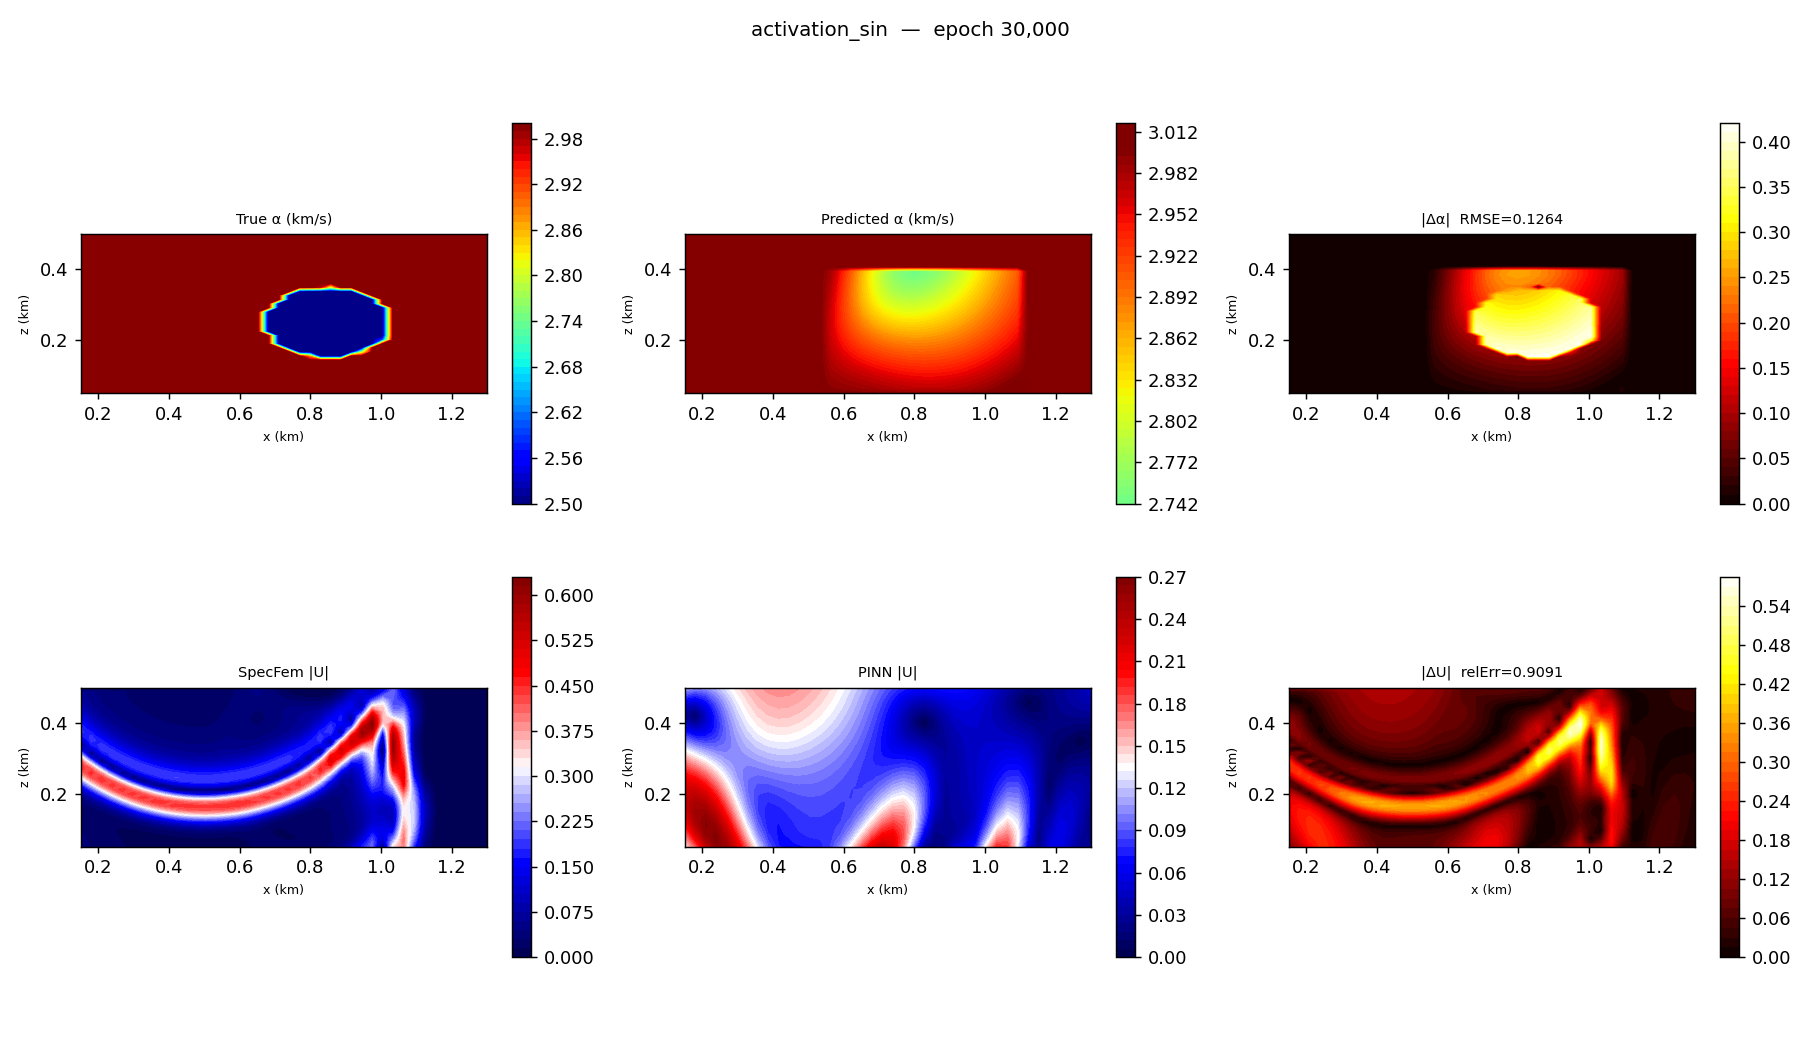
\includegraphics[width=0.8\textwidth]{activation_sin_final.png}
  \caption{Sinusoidal activation results (RMSE = 0.126~km/s).
The anomaly is better resolved with a more clearly defined low-velocity region.}
  \label{fig:sin-activation}
\end{figure}

\textbf{Adaptive tanh activations} fail catastrophically (RMSE = 1.119~km/s).
The wavespeed network collapses to a nearly uniform $\sim$1.0~km/s prediction across the domain (Figure~\ref{fig:adaptive-act}).
The failure mechanism can be understood quantitatively. Since inputs are normalized to $[-1,1]$, a typical pre-activation argument has magnitude $|n \cdot a \cdot x|
\approx n|a|$. For $n = 5$, once $a$ exceeds approximately 0.6 the peak argument reaches 3.0, where $\tanh'(3.0) \approx 0.01$, a 100$\times$ gradient attenuation per layer.
With 4 hidden layers, the effective gradient signal reaching the early layers is attenuated by a factor of roughly $0.01^4 = 10^{-8}$, making meaningful weight updates impossible.
Because $a$ is updated by the same optimizer as the network weights, it grows during the early high-loss phase when gradients are large and noisy;
once the tanh arguments saturate, the vanishing gradients prevent $a$ from recovering.
The coupled inverse problem exacerbates this: the wavespeed network's collapse feeds an incorrect velocity into the PDE residual, creating a feedback loop that locks both networks into their failed states.
This pathology does not arise in the forward-only problems studied in \citet{jagtap2020adaptive}, where the target solution is fixed and cannot co-evolve with the activation parameters.
\begin{figure}[H]
  \centering
  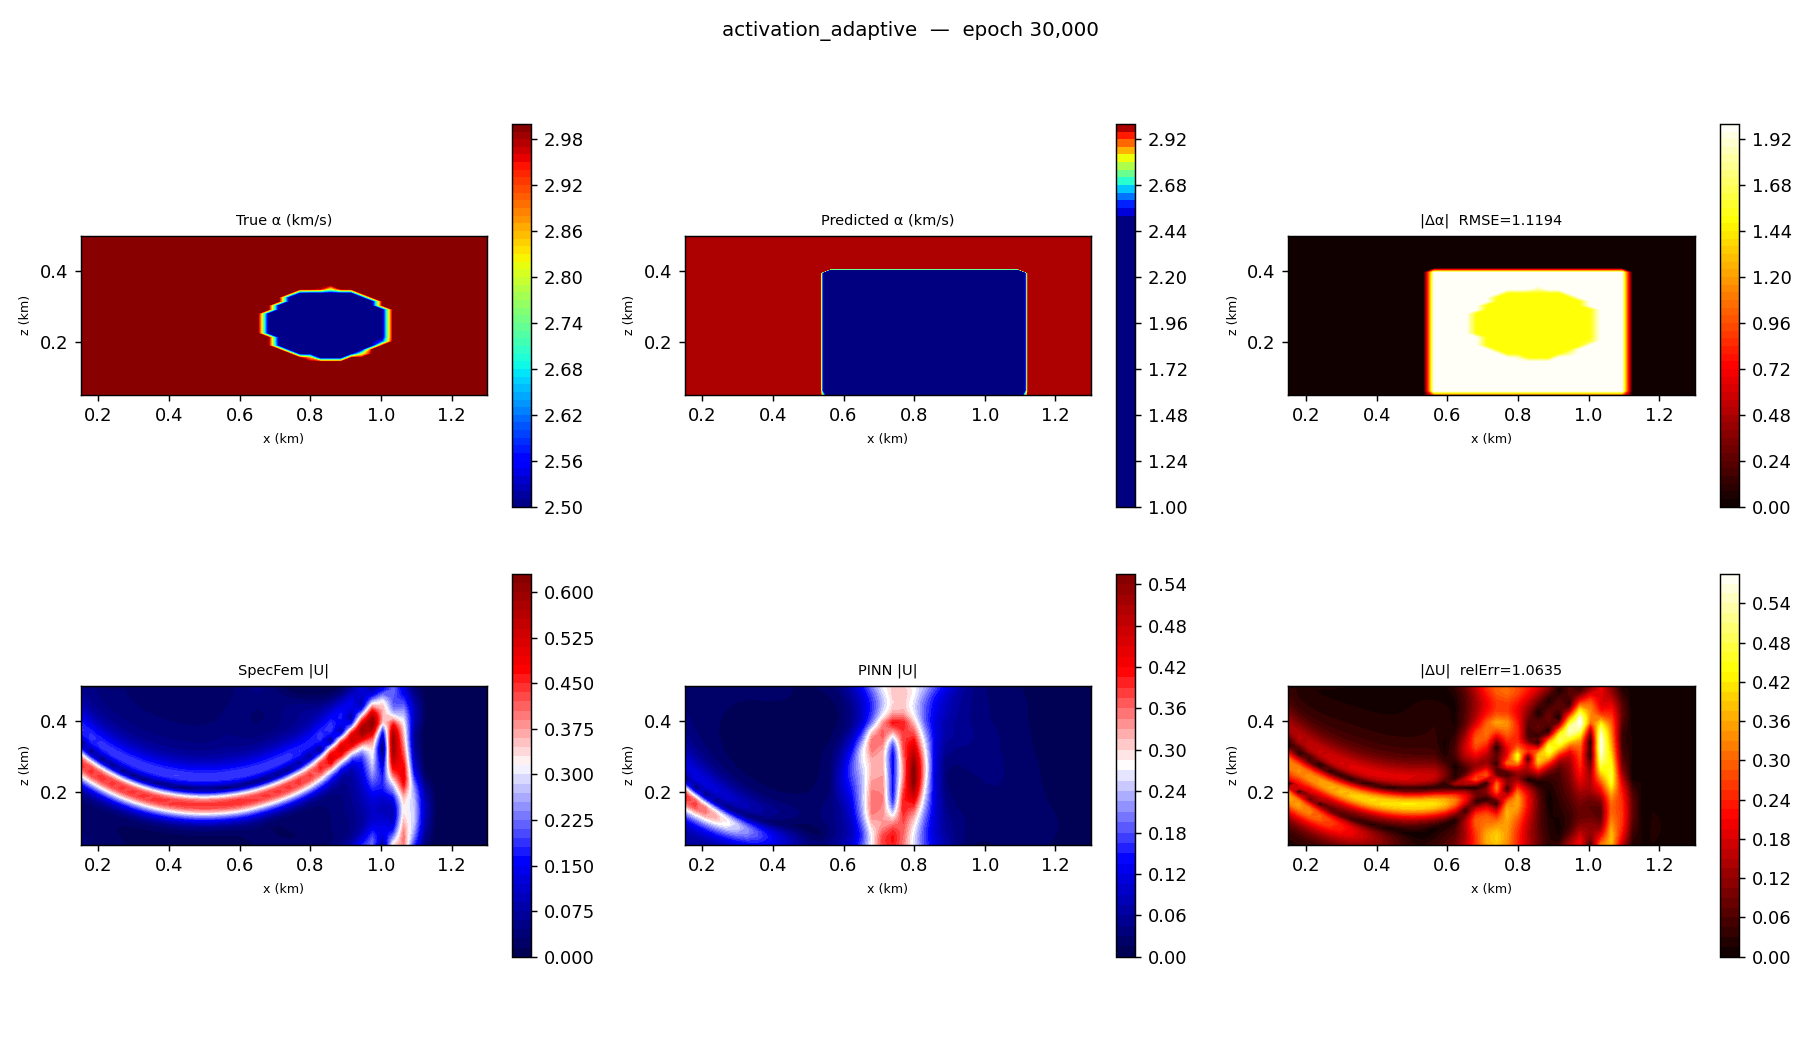
\includegraphics[width=0.8\textwidth]{adaptive_tanh_final.png}
  \caption{Adaptive tanh failure. The scaling parameters saturate early, locking the wavespeed network into a uniform low-velocity prediction (RMSE = 1.119~km/s).}
  \label{fig:adaptive-act}
\end{figure}

\textbf{Fourier feature encoding} degrades velocity recovery (RMSE = 0.229~km/s).
The wavefield shows pronounced striped artifacts at amplitudes $\sim 10^{-3}$, orders of magnitude below the ground truth (Figure~\ref{fig:fourier}).
The RFF encoding with $\sigma = 4.0$ places peak sensitivity at ${\sim}2.9$~cycles/km, a factor of two below the wavefield's dominant spatial frequency of ${\sim}6.7$~cycles/km ($\alpha/f = 3.0/20 = 0.15$~km).
This mismatch amplifies representational capacity in an irrelevant frequency band while allowing the network to fit spurious oscillations consistent with sparse observations but violating the PDE.
Section~\ref{sec:spectral} develops this argument further.

\begin{figure}[H]
  \centering
  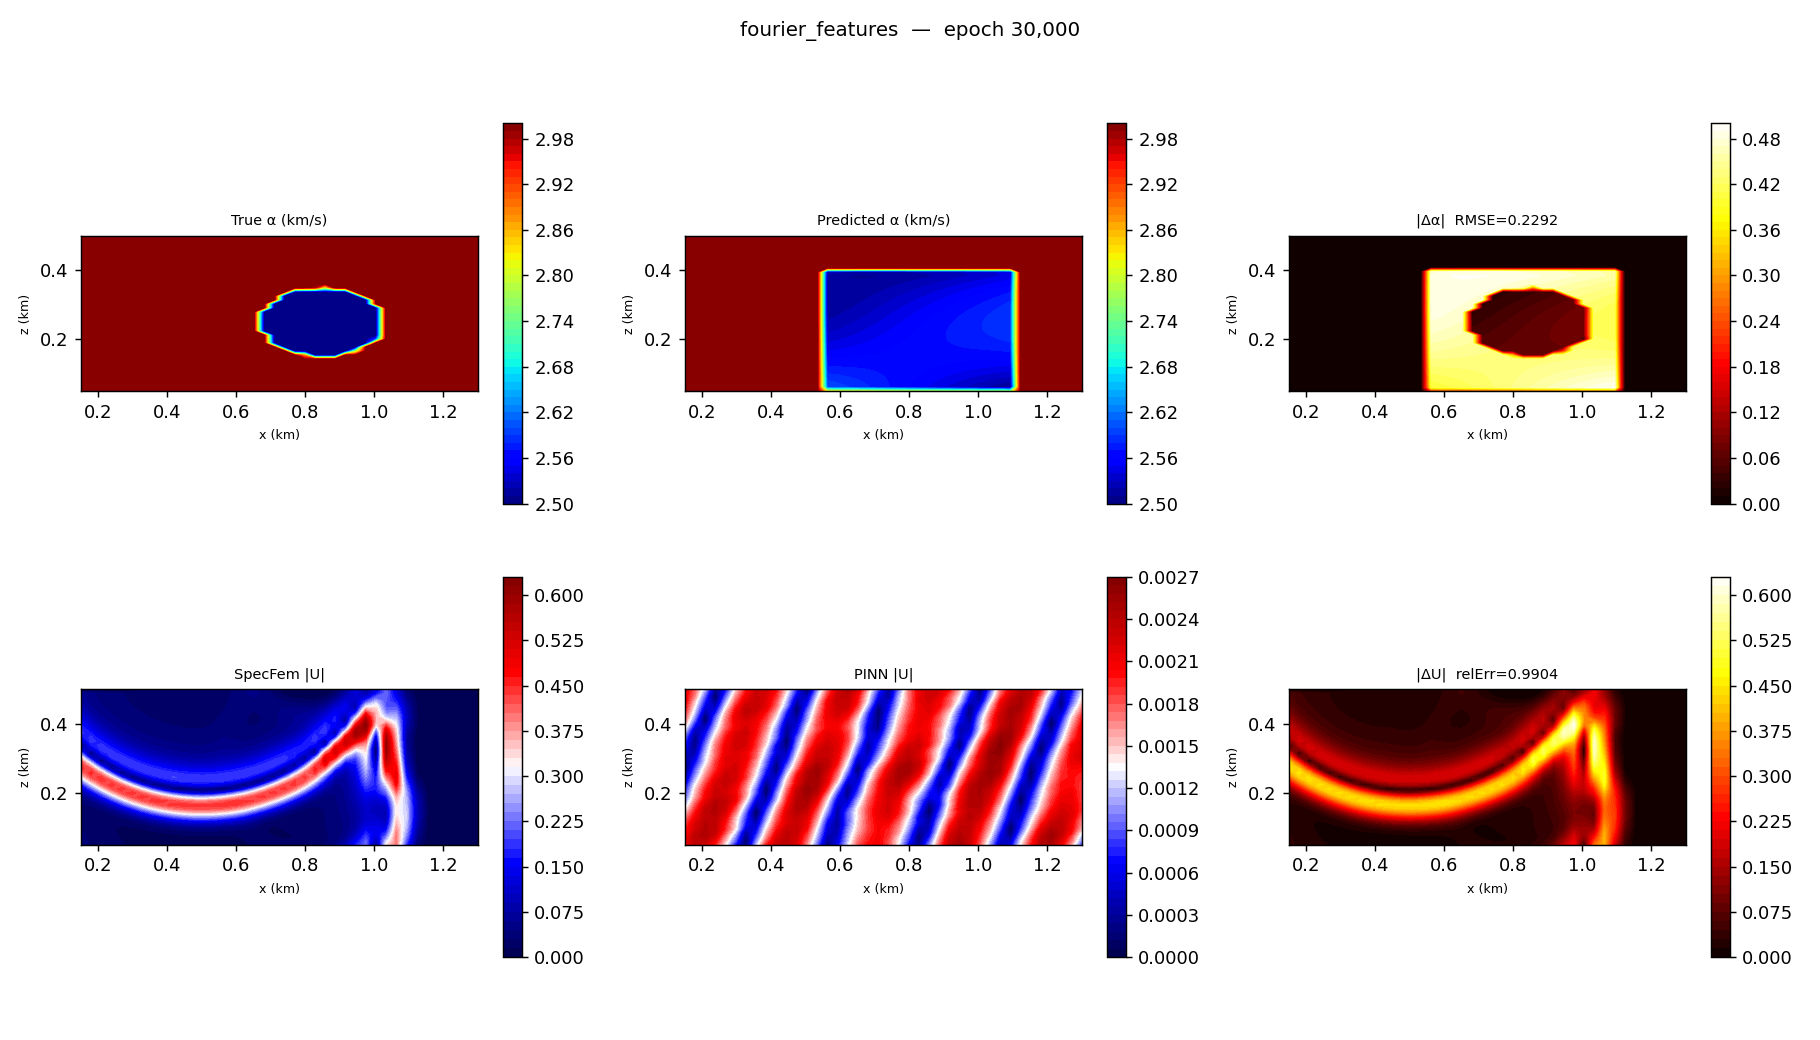
\includegraphics[width=0.8\textwidth]{fourier_features_final.png}
  \caption{Fourier feature results.
The anomaly shape is sharper but the wavefield is dominated by spurious oscillations at ${\sim}10^{-3}$ amplitude.}
  \label{fig:fourier}
\end{figure}

\textbf{Adaptive collocation} achieves the best RMSE (0.125~km/s) with the shortest training time (1162~s, Figure~\ref{fig:adaptive-colloc}), as concentrating points near high-residual regions enforces the PDE more efficiently.
However, the wavefield relative error (1.026) is higher than the baseline, a tradeoff explored in Section~\ref{sec:wavefield-gap}.
\begin{figure}[H]
  \centering
  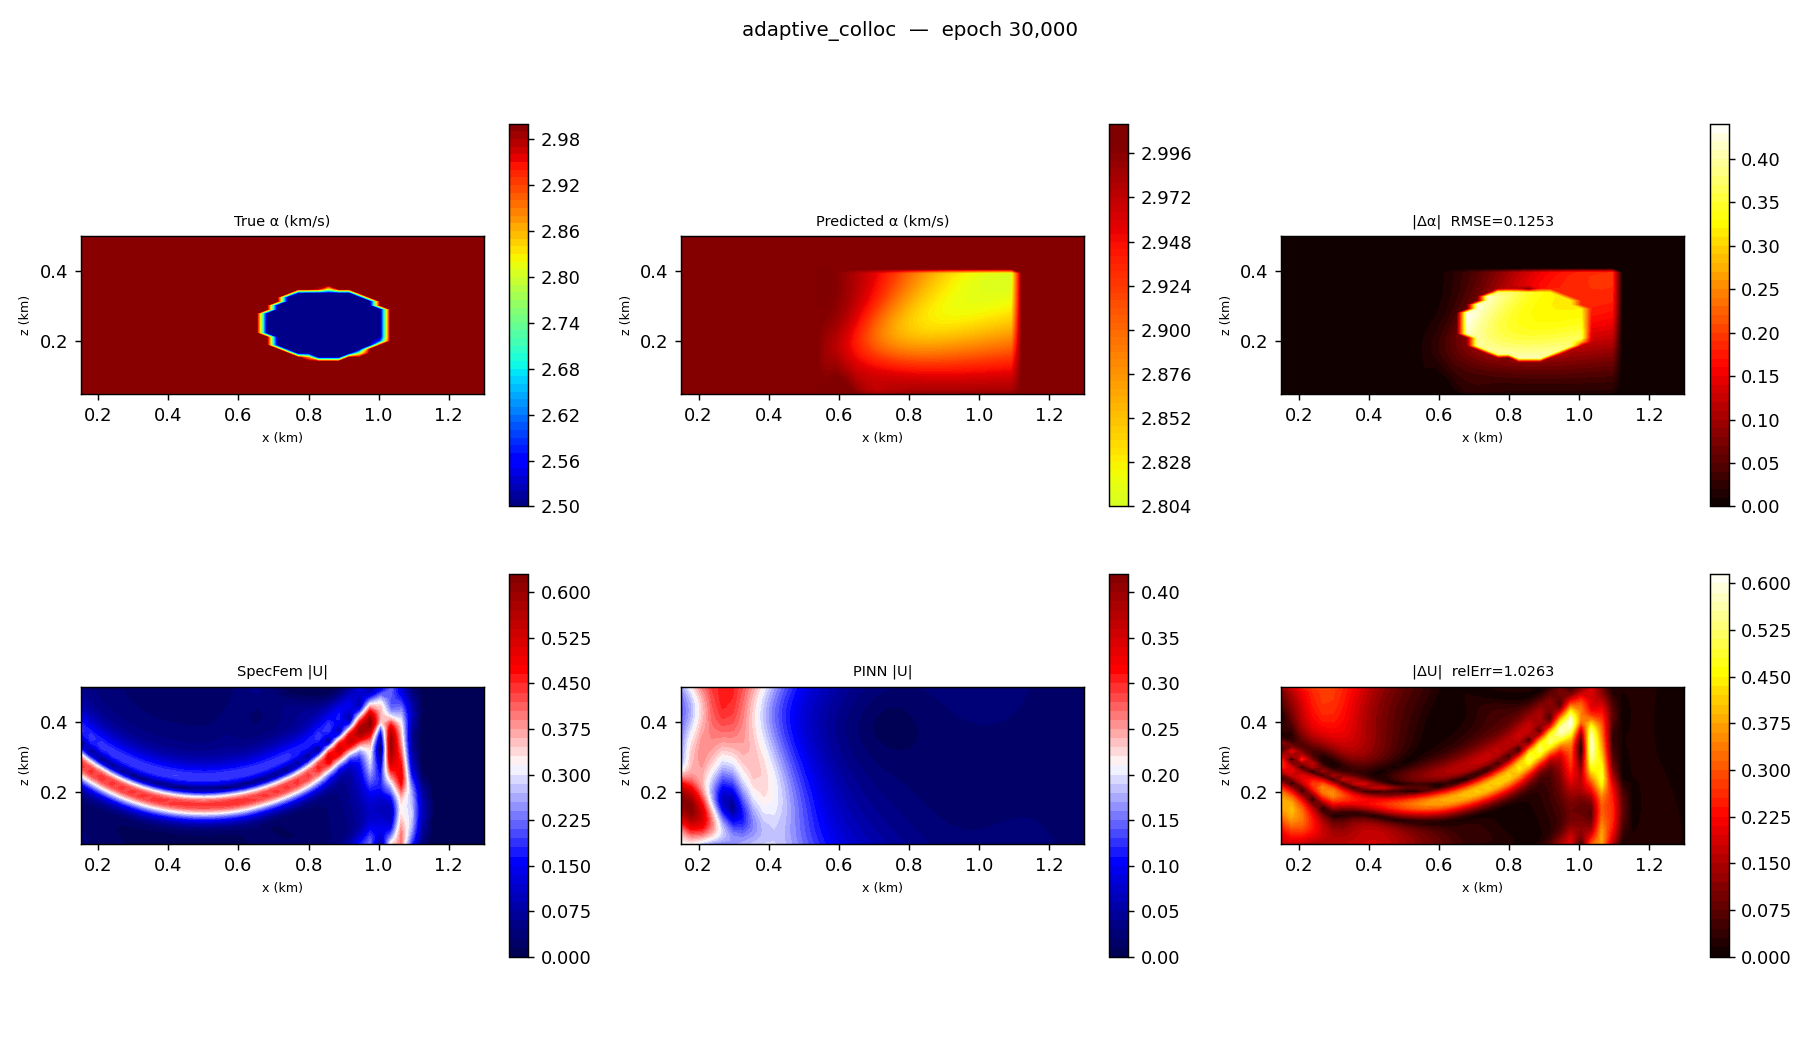
\includegraphics[width=0.8\textwidth]{adaptive_colloc_final.png}
  \caption{Adaptive collocation results (RMSE = 0.125~km/s).}
  \label{fig:adaptive-colloc}
\end{figure}

\subsection{Convergence}
\label{sec:convergence}

Figure~\ref{fig:loss-comparison} compares training loss and RMSE trajectories.
Successful runs converge rapidly by $\sim$10{,}000 epochs; the adaptive activation and Fourier feature runs plateau at substantially higher loss values.
\begin{figure}[H]
  \centering
  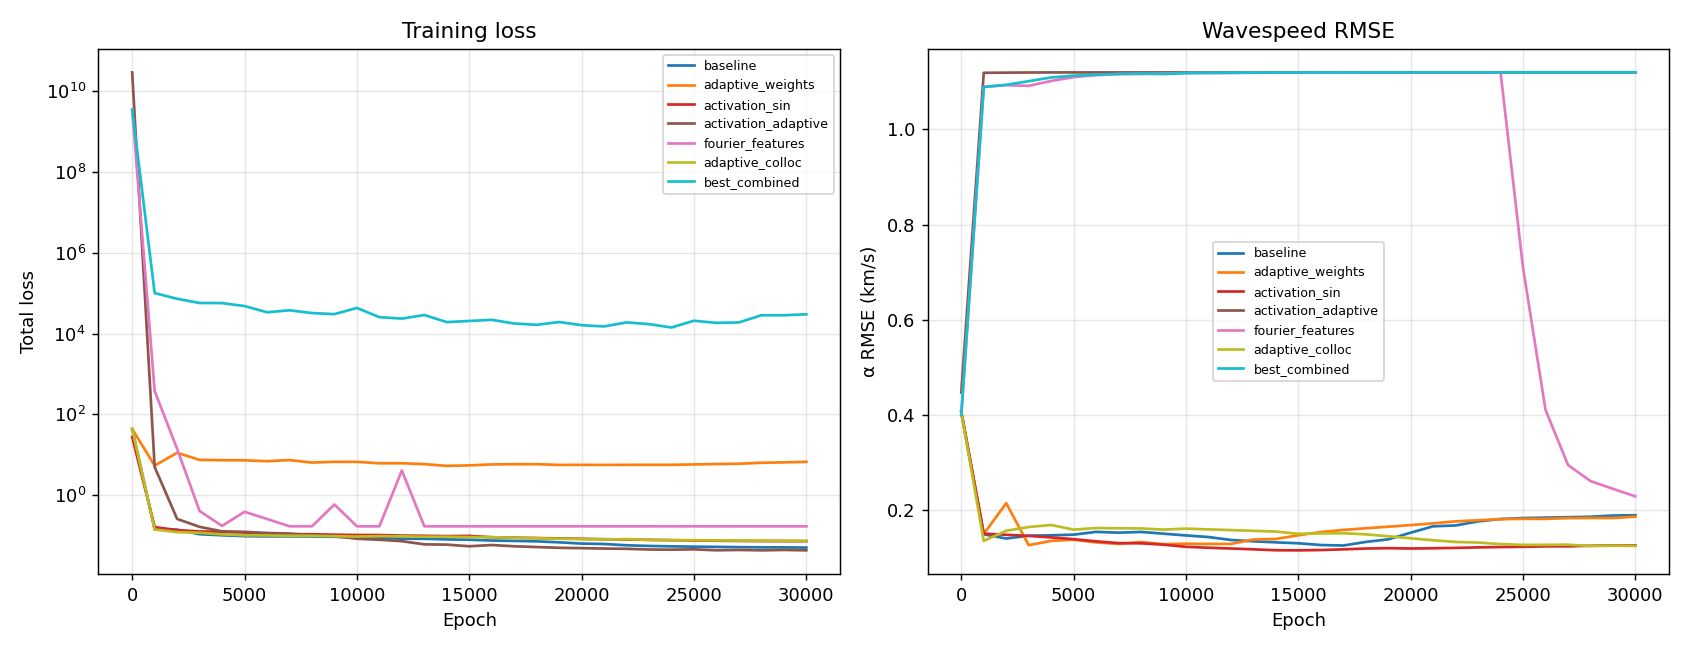
\includegraphics[width=0.8\textwidth]{loss_comparison.png}
  \caption{Training loss (left, log scale) and wavespeed RMSE (right) vs.\ epoch.}
  \label{fig:loss-comparison}
\end{figure}

\section{Discussion}
\label{sec:discussion}

\subsection{Comparison with the Original Study}
\label{sec:comparison-original}

Direct quantitative comparison with \citet{rashtbehesht2022} is difficult: the original reports Case~3 results qualitatively rather than as numerical RMSE values, and several setup differences (SpecFem2D with PML vs.\ our FD solver with sponge layers; 5-layer sin-activation network trained for 400{,}000 iterations with Adam + L-BFGS vs.\ our 4-layer tanh baseline at 30{,}000 Adam epochs) preclude matching absolute numbers.
The original notes that a smaller network ``still yields a good estimate of the wavespeed distribution, however the recovered wavefield is less accurate,'' which is qualitatively consistent with our baseline (RMSE = 0.190~km/s, wavefield relative error 0.875).
Our absolute values should therefore not be read as a reproduction of the original's performance.
The baseline instead establishes a controlled reference against which improvements are evaluated under identical conditions;
the relative rankings, which are the primary contribution, are internally valid provided the improvements interact with problem structure rather than solver-specific artifacts.

\subsection{Spectral Interpretation of Activation and Encoding Effects} \label{sec:spectral}
The contrasting outcomes can be understood through the neural tangent kernel (NTK) \citep{jacot2018neural}.
The NTK eigenvalue spectrum controls which frequency components are learned first;
for tanh networks, eigenvalues decay rapidly with frequency, producing spectral bias toward low-frequency solutions.
Sinusoidal activations introduce periodic structure into $\nabla_\Theta f$, flattening the eigenvalue decay and allowing high-frequency components to be learned at comparable rates.
This explains the improved wavespeed recovery at the anomaly boundary, where spatial frequency content is ${\sim}5.6$~cycles/km.
Fourier feature encoding achieves a similar modification but with less control: the RFF bandwidth set by $\sigma = 4.0$ places peak sensitivity at ${\sim}2.9$~cycles/km, misaligned with both the anomaly scale and the wavefield's dominant spatial frequency (${\sim}6.7$~cycles/km).
A principled choice $\sigma \approx fL_x/\alpha = 9.3$ would better match the wavefield spectrum.
Adaptive collocation does not modify spectral properties but concentrates the PDE constraint near high-residual regions (wavefronts, material interfaces), achieving a similar practical effect through a complementary mechanism operating on the loss landscape rather than the architecture.

\subsection{The Velocity--Wavefield Error Gap}
\label{sec:wavefield-gap}

A striking pattern in Table~\ref{tab:results} is that every run has wavefield relative error above 0.87, and the two best velocity runs actually produce \emph{worse} wavefield errors than the baseline.
This reflects a structural tension in the coupled optimization: the wavefield network must simultaneously match observations and satisfy the PDE with whatever velocity the wavespeed network currently predicts.
Early in training the velocity is poor, so the network learns a compromise;
as velocity improves, the wavefield must unlearn this compromise by traversing a high-loss region.
Improvements that accelerate velocity convergence (sin activations, adaptive collocation) exacerbate this: the velocity changes faster than the wavefield can track.
This suggests the error is a training dynamics issue rather than a capacity limitation, and that staged training, involving first fitting the forward problem and then gradually introducing the velocity as learnable, might help.

\subsection{Limitations}
\label{sec:limitations}

Our second-order FD solver may introduce numerical dispersion absent from the original's spectral element solver.
The networks are small (4 layers, 50 neurons) relative to \citet{rashtbehesht2022}; improvement effectiveness may change at scale.

We test a single synthetic configuration and train for 30{,}000 epochs versus up to 400{,}000 in the reference.
With each run requiring 20--23 minutes on a single NVIDIA RTX 4070 (Table~\ref{tab:results}), a combinatorial sweep over improvements and hyperparameters was not feasible within our compute budget.

\section{Conclusion}
\label{sec:conclusion}

Among four proposed improvements to the PINN-based FWI framework of \citet{rashtbehesht2022}, sinusoidal activations and adaptive collocation each reduce wavespeed RMSE by $\sim$34\%, while adaptive loss weighting provides minimal benefit and Fourier features degrade performance.
Adaptive tanh activations fail due to a saturation feedback loop specific to coupled inverse problems.
The most unexpected finding is that better velocity recovery does not imply better wavefield reconstruction.
The velocity--wavefield error gap suggests that the coupled optimization has fundamentally different dynamics than a pure forward PINN: the wavefield network must track a moving target as the velocity evolves, and faster velocity convergence can actually destabilize this tracking.
For practitioners starting a PINN-based inversion project, this has a concrete implication: monitoring velocity RMSE alone is insufficient, and a staged training curriculum that decouples the forward and inverse problems during early epochs may be necessary.

More broadly, our results reinforce that PINN training enhancements cannot be treated as interchangeable plug-ins.
Each interacts with the problem structure in ways that theoretical motivation alone does not predict.
Systematic ablation on the specific problem at hand remains essential.

A natural next step is to combine the two successful improvements.
Because sinusoidal activations and adaptive collocation operate on orthogonal aspects of the training (network representational capacity versus loss sampling efficiency), we hypothesize that their benefits should compose nearly additively.
The NTK perspective also suggests a principled Fourier feature bandwidth: $\sigma \approx fL/\alpha_0 \approx 9.3$ for our configuration, which would test whether the encoding's failure is fundamental or merely a tuning issue.
\clearpage

\begin{thebibliography}{99}
\bibitem[Jacot et~al.(2018)]{jacot2018neural}
Jacot, A., Gabriel, F., \& Hongler, C. (2018).
Neural tangent kernel: Convergence and generalization in neural networks.
In \textit{Advances in Neural Information Processing Systems} (Vol.~31).
\url{https://doi.org/10.48550/arXiv.1806.07572}

\bibitem[Jagtap et~al.(2020)]{jagtap2020adaptive}
Jagtap, A.~D., Kawaguchi, K., \& Karniadakis, G.~E. (2020).
Adaptive activation functions accelerate convergence in deep and physics-informed neural networks.
\textit{Journal of Computational Physics}, \textit{404}, 109136.
\url{https://doi.org/10.1016/j.jcp.2019.109136}

\bibitem[Raissi et~al.(2019)]{raissi2019physics}
Raissi, M., Perdikaris, P., \& Karniadakis, G.~E. (2019).
Physics-informed neural networks: A deep learning framework for solving forward and inverse problems involving nonlinear partial differential equations.
\textit{Journal of Computational Physics}, \textit{378}, 686--707.
\url{https://doi.org/10.1016/j.jcp.2018.10.045}

\bibitem[Rasht-Behesht et~al.(2022)]{rashtbehesht2022}
Rasht-Behesht, M., Huber, C., Shukla, K., \& Karniadakis, G.~E. (2022).
Physics-informed neural networks (PINNs) for wave propagation and full waveform inversions.
\textit{Journal of Geophysical Research: Solid Earth}, \textit{127}(5), e2021JB023120.
\url{https://doi.org/10.1029/2021JB023120}

\bibitem[Sitzmann et~al.(2020)]{sitzmann2020implicit}
Sitzmann, V., Martel, J.~N.~P., Bergman, A.~W., Lindell, D.~B., \& Wetzstein, G. (2020).
Implicit neural representations with periodic activation functions.
In \textit{Advances in Neural Information Processing Systems} (Vol.~33, pp.~7462--7473).
\url{https://doi.org/10.48550/arXiv.2006.09661}

\bibitem[Tancik et~al.(2020)]{tancik2020fourier}
Tancik, M., Srinivasan, P.~P., Mildenhall, B., Fridovich-Keil, S., Raghavan, N., Singhal, U., Ramamoorthi, R., Barron, J.~T., \& Ng, R. (2020).
Fourier features let networks learn high frequency functions in low dimensional domains.
In \textit{Advances in Neural Information Processing Systems} (Vol.~33, pp.~7537--7547).
\url{https://doi.org/10.48550/arXiv.2006.10739}

\bibitem[Wang et~al.(2021)]{wang2021understanding}
Wang, S., Teng, Y., \& Perdikaris, P. (2021).
Understanding and mitigating gradient flow pathologies in physics-informed neural networks.
\textit{SIAM Journal on Scientific Computing}, \textit{43}(5), A3055--A3081.
\url{https://doi.org/10.1137/20M1318043}

\end{thebibliography}

\end{document}